\documentclass[conference]{IEEEtran}
\IEEEoverridecommandlockouts
\usepackage{cite}
\usepackage{amsmath,amssymb}
\usepackage{graphicx}
\usepackage{booktabs}
\usepackage{xcolor}
\usepackage{textcomp}
\usepackage[T1]{fontenc}
\usepackage{url}
\newcommand{\HkN}{10{,}000}
\newcommand{\HkUnique}{743}
\newcommand{\HkDupPct}{92.6\%}
\newcommand{\HkTopCount}{60}
\newcommand{\HkUrgAuc}{1.000}
\newcommand{\HkTrivAuc}{0.984}
\newcommand{\HkFirstAuc}{0.665}
\newcommand{\HkRandAuc}{1.000}
\newcommand{\HkGroupAuc}{1.000}
\newcommand{\HamN}{14{,}000}
\newcommand{\HamMasked}{5{,}461}
\newcommand{\HamMaskedPct}{39.0\%}
\newcommand{\HamExactDupPct}{7.9\%}
\newcommand{\HamTestN}{1{,}400}
\newcommand{\HamTestUnique}{1{,}399}
\newcommand{\HamTestNN}{0.07\%}
\newcommand{\HamTestExact}{0.0\%}
\newcommand{\HamRandAuc}{1.000}
\newcommand{\HamGroupAuc}{0.999}
\newcommand{\HamTrivHigh}{10}
\newcommand{\HamTrivMin}{0.584}
\newcommand{\HamTrivMinLang}{Assamese}
\newcommand{\HamLowN}{6}
\newcommand{\HamLowMax}{44}
\newcommand{\HamLowMin}{38}
\newcommand{\TrHkHam}{0.951}
\newcommand{\TrHamHk}{0.984}
\newcommand{\IcfdTrN}{21{,}000}
\newcommand{\IcfdTrFraud}{30.9\%}
\newcommand{\IcfdTrNormal}{14{,}519}
\newcommand{\IcfdVaN}{4{,}500}
\newcommand{\IcfdVaFraud}{99.4\%}
\newcommand{\IcfdVaNormal}{26}
\newcommand{\IcfdTeN}{4{,}500}
\newcommand{\IcfdTeFraud}{99.5\%}
\newcommand{\IcfdTeNormal}{23}
\newcommand{\IcfdCdN}{1{,}000}
\newcommand{\IcfdCdFraud}{96.1\%}
\newcommand{\IcfdCdNormal}{39}
\newcommand{\IcfdAllFraudAcc}{99.5\%}
\newcommand{\IcfdAllFraudF}{99.7\%}
\newcommand{\IcfdAllFraudCi}{14\%}
\newcommand{\IcfdTrNormalNA}{97.7\%}
\newcommand{\IcfdTeNormalFailed}{22}
\newcommand{\IcfdCvAuc}{0.995}
\newcommand{\IcfdTeAuc}{0.822}
\newcommand{\IcfdVaAuc}{0.855}
\newcommand{\IcfdCdAuc}{0.860}
\newcommand{\IcfdTeFpr}{35\%}
\newcommand{\IcfdTeFpLo}{19\%}
\newcommand{\IcfdTeFpHi}{55\%}
\newcommand{\IcfdTeFp}{8}
\newcommand{\IcfdTeNormN}{23}
\newcommand{\IcfdCvFpr}{2.3\%}
\newcommand{\IcfdTeAcc}{86.5\%}
\newcommand{\IcfdFirstTurnTe}{4.5\%}
\newcommand{\IcfdNNTe}{0.0\%}
\newcommand{\InN}{9{,}487}
\newcommand{\InLangs}{10}
\newcommand{\InFiles}{18{,}974}
\newcommand{\InChinaPct}{42.4\%}
\newcommand{\InIndiaN}{0}
\newcommand{\InChinaN}{8{,}046}
\newcommand{\RdScanned}{226{,}000}
\newcommand{\RdMatched}{6{,}005}
\newcommand{\RdCand}{243}
\newcommand{\RdVerb}{12}
\newcommand{\RdDeva}{0}
\newcommand{\MuHamIid}{1.000}
\newcommand{\MuHkIid}{1.000}
\newcommand{\MuHamOff}{0.928}
\newcommand{\MuHamOffTpr}{63\%}
\newcommand{\MuHamToHk}{0.918}
\newcommand{\MuHamToHkTpr}{25\%}
\newcommand{\MuHkToHinglish}{0.995}
\newcommand{\MuHkToOff}{0.826}
\newcommand{\MuHkToOffFpr}{64\%}
\newcommand{\MuHkToOtherLo}{0.752}
\newcommand{\MuHkToOtherHi}{0.785}
\newcommand{\MuHkToOtherFprLo}{86\%}
\newcommand{\MuHkToOtherFprHi}{88\%}
\newcommand{\XlHamIid}{1.000}
\newcommand{\XlHkIid}{1.000}
\newcommand{\XlHamOff}{0.972}
\newcommand{\XlHamOffTpr}{83\%}
\newcommand{\XlHamToHk}{0.929}
\newcommand{\XlHamToHkTpr}{42\%}
\newcommand{\XlHkToHinglish}{0.992}
\newcommand{\XlHkToOff}{0.828}
\newcommand{\XlHkToOffFpr}{56\%}
\newcommand{\XlHkToOtherLo}{0.714}
\newcommand{\XlHkToOtherHi}{0.825}
\newcommand{\XlHkToOtherFprLo}{77\%}
\newcommand{\XlHkToOtherFprHi}{84\%}


\begin{document}

\title{How Much Do Benchmark Scores Tell Us? An Audit of Public Datasets for Scam Detection in Indian Languages}

\author{\IEEEauthorblockN{Aryan Chaurasia}
\IEEEauthorblockA{\textit{Department of Information Technology} \\
\textit{K. J. Somaiya College of Engineering}\\
Mumbai, India \\
aryan.chaurasia@somaiya.edu}}

\maketitle

\begin{abstract}
Several public datasets now support scam detection in Indian languages, and models reach near-perfect scores on them. We audit four of them (a 10{,}000-row Hinglish utterance set, a 14-language message set, the ICFD-31k conversation set and the text of INDICA) for provenance, redundancy, shortcut features, split design and transfer. The Hinglish set holds only \HkUnique{} distinct texts in \HkN{} rows, and its \texttt{urgency\_level} field alone separates the classes (AUROC \HkUrgAuc). In the 14-language set, \HamLowN{} languages have \HamLowMin{}--\HamLowMax{} distinct templates per 1{,}000 rows, and message length, digit and link counts alone reach AUROC of at least 0.98 in \HamTrivHigh{} languages. In the released ICFD-31k files the validation and test splits are \IcfdTeFraud{} fraud, so the test set contains \IcfdTeNormal{} normal conversations and cannot measure false alarms; a constant ``fraud'' prediction scores \IcfdAllFraudAcc{} accuracy. The INDICA text is one set of \InN{} items machine-translated into \InLangs{} languages, and none of its \InFiles{} English files contains a marker of Indian context such as UPI, Aadhaar or rupees, whereas \InChinaPct{} contain China-specific markers. Fine-tuned MuRIL and XLM-R score AUROC \MuHamIid{} and \XlHamIid{} on held-out templates but score lower on the dataset's own official test and on the other datasets. A search of \RdScanned{} public Reddit posts recovered only \RdVerb{} verbatim scam utterances, none multi-turn or in Devanagari. We close with a reporting checklist for scam-detection datasets.
\end{abstract}

\begin{IEEEkeywords}
scam detection, Indian languages, Hinglish, dataset audit, benchmark validity, shortcut learning
\end{IEEEkeywords}

\section{Introduction}
Online scams reach people in their own languages: a caller who impersonates a police officer in Hindi, a ``task'' job offer in Hinglish, an electricity-disconnection message in Marathi. Detection systems for these settings need training and test data, and real conversations are hard to obtain and raise privacy concerns when shared. Researchers have therefore turned to datasets that are generated, translated or only loosely documented. Recent releases cover English and Hinglish phone calls~\cite{ahuja2026icfd}, ten Indian languages~\cite{indicadata}, and short scam messages in 14 languages~\cite{ham14data}. The ICFD-31k README, for example, reports 99.6 accuracy and F1 for a fine-tuned classifier.

A high score on a benchmark is only informative if the benchmark can separate good models from bad ones, covers the situations the system will face, and measures what its name says. Work on natural language inference showed that classifiers can reach well above chance by looking only at the hypothesis~\cite{gururangan2018annotation,poliak2018hypothesis}, and that datasets written by LLMs carry their own artifacts~\cite{proebsting2024hypothesis}. More generally, models learn shortcuts that work on a benchmark and fail elsewhere~\cite{geirhos2020shortcut}. We ask whether the public scam-detection datasets for Indian languages are subject to these problems, using only the released files and public tools.

We make four contributions.
\begin{itemize}
\item \textbf{An audit protocol and results for four datasets.} We measure documented provenance, exact and template-level redundancy, trivial-feature and metadata shortcuts, train/test overlap, split class balance and cross-dataset transfer (Sections~\ref{sec:method} and~\ref{sec:results}).
\item \textbf{Concrete defects, each reproducible from the released files.} Among them: \HkDupPct{} exact duplicates in one dataset; a test split with \IcfdTeNormal{} negatives in another; and a ten-language set whose English side contains none of our Indian-context markers.
\item \textbf{A transfer experiment with two multilingual encoders.} Held-out-template scores are saturated, while the dataset's own test set and other datasets give lower and less stable scores.
\item \textbf{A negative result on real data.} Mining public forum posts yields too few verbatim scam messages to build a test set, which is itself a finding about data availability, and a reporting checklist.
\end{itemize}
We do not claim that any model trained on these sets is useless, or that the authors acted in bad faith. Several datasets say plainly that they are synthetic. Our point is narrower: the numbers they produce should not be read as evidence about real-world scam detection.

\section{Related Work}
\textbf{Scam and fraud detection from conversations.} Shen et al.\ model scam calls and warn users in real time with an LLM~\cite{shen2025warned}. PreScam builds 11{,}573 conversation instances from user-submitted scam reports and predicts how a scam will progress~\cite{sun2026prescam}. ScriptMind fine-tunes small models on 571 Korean phone-scam cases~\cite{kim2026scriptmind}. TeleAntiFraud-28k provides audio-text telecom fraud data~\cite{ma2025teleantifraud}. Closest to our setting, ICFD-31k provides 31{,}000 synthetic English and Hinglish call transcripts with streaming labels~\cite{ahuja2026icfd}, and Rani et al.\ classify Hinglish cybercrime complaints~\cite{rani2024cybercrime}. We found no prior audit of how well these resources support claims about Indian-language scams.

\textbf{Artifacts and shortcuts.} Hypothesis-only baselines expose annotation artifacts in NLI data~\cite{gururangan2018annotation,poliak2018hypothesis}; the same check on LLM-written hypotheses finds artifacts too~\cite{proebsting2024hypothesis}. Geirhos et al.\ describe shortcut learning as a common failure that benchmarks hide~\cite{geirhos2020shortcut}. Our trivial-feature and metadata baselines follow the same logic.

\textbf{Synthetic data as training and test data.} LLM-generated data helps classification least when the task is subjective~\cite{li2023synthetic}, can differ from the target distribution unless it is grounded~\cite{veselovsky2023faithful}, and tracks real-data performance for simple tasks better than for complex ones when used as a benchmark~\cite{maheshwari2024efficacy}. Scam detection depends on subtle social cues, so these cautions apply.

\textbf{Indic language models.} MuRIL~\cite{khanuja2021muril} and XLM-R~\cite{conneau2020xlmr} are standard multilingual encoders for Indian languages, and HingBERT targets Hindi--English code-mixing~\cite{nayak2022hingbert}. We use the first two as probes.

\section{Datasets Audited}
\label{sec:data}
Table~\ref{tab:data} summarizes what each dataset's public documentation says about how it was made. H10k and Ham14 are our short names for the two Hugging Face sets described below.

\begin{table*}[t]
\centering
\caption{Datasets audited and what their public documentation states about provenance (checked October 2026).}
\label{tab:data}
\small
\begin{tabular}{p{1.9cm}p{2.7cm}p{2.5cm}p{4.2cm}p{4.2cm}}
\toprule
Short name & Unit and size & Languages & Stated provenance & Audited here \\
\midrule
H10k~\cite{h10kdata} & single utterances, 10{,}000 rows, with category, caller type, urgency and duration fields & Hinglish (card also lists English and Hindi) & Card does not say how the data were collected & Duplicates, metadata and trivial-feature shortcuts, transfer \\
Ham14~\cite{ham14data} & single messages, 14{,}000 rows plus a 1{,}400-row test file & 14 languages incl.\ Hindi, Marathi, Hinglish, English & ``Realistic communication patterns''; no collection method given & Per-language redundancy, shortcuts, test overlap, transfer \\
ICFD-31k~\cite{ahuja2026icfd} & call transcripts, 31{,}000 & English, Hinglish & Synthetic (dataset card) & Split balance, normal-class meaning, redundancy, baseline \\
INDICA text~\cite{indicadata} & text of calls, \InN{} items $\times$ \InLangs{} languages & 10 Indian languages & Built on TeleAntiFraud-28k per file names; the card says it builds on the IndiF set; creation not described & Parallelism, context markers \\
\bottomrule
\end{tabular}
\end{table*}

We also looked at MultiFraudAlign~\cite{mfadata}, which states that it is fully synthetic and was generated with Qwen2.5-72B, but did not audit it.

\section{Method}
\label{sec:method}
\textbf{Masking and templates.} We lower-case text, replace digit runs (in any Indic script) with a placeholder, replace links, and collapse white space. Two rows with the same masked text belong to one template. This is a conservative notion: paraphrases of one template count as different.

\textbf{Redundancy.} We report exact duplicates, distinct templates, and, for train/test pairs, the share of test rows whose nearest training row has character $n$-gram TF-IDF cosine similarity of at least 0.9.

\textbf{Shortcuts.} We fit logistic regression (five-fold cross-validation) on features that should carry little scam semantics: text length, digit count, link presence, punctuation count and word count; on the first word alone; and, where present, on metadata fields. We also fit a character $n$-gram TF-IDF classifier with random folds and with folds grouped by template.

\textbf{Split design.} For ICFD-31k we count the labels in each released split and the \texttt{scam\_outcome} field, and compare a constant ``fraud'' predictor and a TF-IDF classifier trained on the released training set across splits. Intervals for rates on small groups are Wilson 95\% intervals~\cite{wilson1927}.

\textbf{Parallelism and context.} For INDICA we compare item identifiers across language folders, and count English files that match a list of China-specific markers (for example WeChat, Alipay, yuan, common Chinese surnames used as titles, public security bureau) or of India-specific markers (UPI, Aadhaar, rupee, PAN card, IFSC, Paytm, PhonePe, large Indian bank names, large Indian cities, lakh, crore). Both lists are in the code release and are heuristics.

\textbf{Transfer with fine-tuned encoders.} We fine-tune MuRIL-base and XLM-R-base for binary classification (3 epochs, learning rate $3\times10^{-5}$, batch size 32, maximum 128 tokens, three seeds) on H10k or on Ham14, using an 80/20 split grouped by template. We then score held-out templates, the Ham14 official test file, the other dataset, and per-language slices. We report AUROC averaged over seeds, with a bootstrap 95\% interval over test items, and the true-positive and false-positive rates at the fixed threshold 0.5. Scikit-learn~\cite{pedregosa2011sklearn} and bootstrap resampling~\cite{efron1979bootstrap} are used throughout. Training ran on a cloud A10G GPU.

\textbf{Public-forum route.} We paged through public posts of four Indian subreddits via a public research archive of Reddit data, kept posts matching scam-related keywords, extracted quoted text, and counted the quotes that one reviewer judged to be a verbatim scam message or call line. The raw text is not released (Section~\ref{sec:ethics}).

\section{Results}
\label{sec:results}

\subsection{H10k: few distinct texts and a metadata leak}
H10k has \HkN{} rows but \HkUnique{} distinct texts (\HkDupPct{} of rows are exact duplicates); the most frequent text appears \HkTopCount{} times. A classifier scores AUROC \HkRandAuc{} with random folds and \HkGroupAuc{} with template-grouped folds, so grouping removes nothing because the classes differ in vocabulary. The \texttt{urgency\_level} field alone gives AUROC \HkUrgAuc{}: every benign row has ``low'' urgency and every scam row ``medium'' or ``high''. Length, digit and link features alone give \HkTrivAuc{}. Fine-tuned MuRIL and XLM-R score \MuHkIid{} and \XlHkIid{} on held-out templates. A score of 1.000 on this set cannot distinguish a good detector from a lookup of surface forms.

\subsection{Ham14: uneven diversity across languages}
Ham14 has \HamN{} rows and \HamMasked{} distinct templates (\HamMaskedPct{}). The spread across languages is wide: \HamLowN{} languages have only \HamLowMin{}--\HamLowMax{} distinct templates per 1{,}000 rows (Table~\ref{tab:ham}). Template-grouped cross-validation gives AUROC \HamGroupAuc{} (random folds \HamRandAuc{}). Trivial features reach at least 0.98 in \HamTrivHigh{} of 14 languages; the lowest is \HamTrivMin{} (\HamTrivMinLang{}). The official test file is separate from training text (exact overlap \HamTestExact{}, \HamTestNN{} of rows with a near-identical training neighbour) and almost all of its \HamTestN{} rows are distinct (\HamTestUnique{}), so it is more diverse than the training set it ships with. That difference matters in Section~\ref{sec:transfer}.

\begin{table}[t]
\centering
\caption{Ham14: distinct templates per 1{,}000 rows, and AUROC of a classifier that sees only length, digit and link features (five-fold CV).}
\label{tab:ham}
\small
\begin{tabular}{lrr}
\toprule
Language & Templates / 1,000 & Trivial-feature AUROC \\
\midrule
Assamese & 40 & 0.584 \\
Bengali & 823 & 1.000 \\
English & 621 & 0.998 \\
Gujarati & 599 & 0.987 \\
Hindi & 594 & 0.997 \\
Hinglish & 808 & 1.000 \\
Kannada & 40 & 0.790 \\
Kashmiri & 583 & 0.989 \\
Malayalam & 40 & 0.866 \\
Marathi & 596 & 0.988 \\
Odia & 44 & 1.000 \\
Punjabi & 595 & 0.987 \\
Tamil & 38 & 1.000 \\
Telugu & 40 & 0.862 \\
\bottomrule
\end{tabular}

\end{table}

\subsection{ICFD-31k: the test set cannot measure false alarms}
Table~\ref{tab:icfd} gives the label balance of the released splits. Training is \IcfdTrFraud{} fraud, but validation is \IcfdVaFraud{} and test \IcfdTeFraud{}, which leaves \IcfdTeNormal{} normal conversations in the test set. A predictor that always answers ``fraud'' scores \IcfdAllFraudAcc{} accuracy and \IcfdAllFraudF{} F1 on this test set. Its false-alarm rate is 100\%, but with only \IcfdTeNormal{} negatives, even a detector with zero false alarms could only show that its true false-alarm rate is below \IcfdAllFraudCi{} (95\% upper bound). We could not access the authors' evaluation code, and the README does not state which split its 99.6 accuracy refers to, so we make no claim about their protocol; we describe what the released files imply.

\begin{table}[t]
\centering
\caption{ICFD-31k released splits.}
\label{tab:icfd}
\small
\begin{tabular}{lrrr}
\toprule
Split & Conversations & Normal & Fraud \\
\midrule
train & 21{,}000 & 14{,}519 & 30.9\% \\
validation & 4{,}500 & 26 & 99.4\% \\
test & 4{,}500 & 23 & 99.5\% \\
cross domain & 1{,}000 & 39 & 96.1\% \\
\bottomrule
\end{tabular}

\end{table}

``Normal'' also does not mean the same thing in the training and test splits. Of the training normals, \IcfdTrNormalNA{} have \texttt{scam\_outcome} ``N/A'' (no scam was attempted); \IcfdTeNormalFailed{} of the \IcfdTeNormal{} test normals are ``Failed'' (an attempt was made and thwarted). A TF-IDF logistic regression reaches AUROC \IcfdCvAuc{} in cross-validation on the training pool (false-alarm rate \IcfdCvFpr{}), but AUROC \IcfdTeAuc{} on the released test, with \IcfdTeFp{} false alarms on \IcfdTeNormN{} normals (\IcfdTeFpr{}, 95\% interval \IcfdTeFpLo{}--\IcfdTeFpHi{}). The drop is consistent with the shift in what ``normal'' means, though we did not isolate the cause. Whole-transcript overlap is not the issue: no test transcript appears in training, and only \IcfdNNTe{} have a near-identical training neighbour, although \IcfdFirstTurnTe{} of test conversations open with a first turn that also appears (after masking) in training.

\subsection{INDICA: a translation of Chinese-origin calls}
In the text archive, the same \InN{} item identifiers appear in all \InLangs{} language folders with the same label, and each identifier has two files (\InFiles{} files per language). The file names carry the TeleAntiFraud-28k corpus name~\cite{ma2025teleantifraud}. The English renderings contain names such as ``Zhang Manager'' and a bank called ``Agricultural and Commercial Bank''. None of the \InFiles{} English files matches our India markers (\InIndiaN{}), whereas \InChinaN{} (\InChinaPct{}) match China-specific markers. These are heuristic counts and the true share is likely higher. The dataset is Indic in language, but the scams it describes are not set in India, and one set of items repeated in ten languages is one sample, not ten. A model that scores well across its ten languages shows ability to detect a particular set of translated calls, not familiarity with Indian scams.

\subsection{Transfer between datasets}
\label{sec:transfer}
Table~\ref{tab:enc} and Fig.~\ref{fig:audit}c show what happens when the same encoders meet other test sets. On held-out templates both encoders trained on Ham14 score AUROC \MuHamIid{} (MuRIL) and \XlHamIid{} (XLM-R). On the Ham14 official test, the same models score \MuHamOff{} and \XlHamOff{}, and at the 0.5 threshold they detect only \MuHamOffTpr{} and \XlHamOffTpr{} of scams. Applied to H10k, models trained on Ham14 score \MuHamToHk{} and \XlHamToHk{} but detect only \MuHamToHkTpr{} and \XlHamToHkTpr{} of scams at 0.5, so their ranking is informative while their operating point is not.

In the other direction, models trained on H10k score \MuHkToHinglish{} and \XlHkToHinglish{} on the Hinglish slice of Ham14, so the two Hinglish sets agree. On the other Ham14 slices (English, Hindi, Marathi) they score \MuHkToOtherLo{}--\MuHkToOtherHi{} (MuRIL) and \XlHkToOtherLo{}--\XlHkToOtherHi{} (XLM-R) with false-alarm rates of \MuHkToOtherFprLo{}--\MuHkToOtherFprHi{} and \XlHkToOtherFprLo{}--\XlHkToOtherFprHi{}. These are zero-shot cross-script and cross-language tests, since H10k contains only Hinglish, and are not an indictment of either model. They do show that a multilingual encoder trained on one Indian-language scam set does not carry its score to other languages, and that a single in-distribution number would hide this. A TF-IDF model trained on one Hinglish set and tested on the Hinglish part of the other scores \TrHkHam{} and \TrHamHk{} in the two directions, confirming that the two Hinglish sets are close to each other.

\begin{table*}[t]
\centering
\caption{Transfer of fine-tuned encoders (mean AUROC over three seeds; intervals in the released JSON). $^\dagger$ held-out templates of the training source. H10k contains only Hinglish, so for H10k-trained models every column except the Hinglish ones is zero-shot.}
\label{tab:enc}
\small
\begin{tabular}{llcccccccc}
\toprule
Encoder & Trained on & H10k$^\dagger$ & Ham14$^\dagger$ & Ham14 off. & H10k all & Ham14 Hing. & Ham14 Hindi & Ham14 Mar. & Ham14 Eng. \\
\midrule
MuRIL & Ham14 & 0.88 & 1.00 & 0.93 & 0.92 & 1.00 & 1.00 & 1.00 & 1.00 \\
MuRIL & H10k & 1.00 & 0.70 & 0.83 & 1.00 & 1.00 & 0.78 & 0.75 & 0.79 \\
XLM-R & Ham14 & 0.91 & 1.00 & 0.97 & 0.93 & 1.00 & 1.00 & 1.00 & 1.00 \\
XLM-R & H10k & 1.00 & 0.68 & 0.83 & 1.00 & 0.99 & 0.71 & 0.74 & 0.83 \\
\bottomrule
\end{tabular}

\end{table*}

\begin{figure*}[t]
\centering
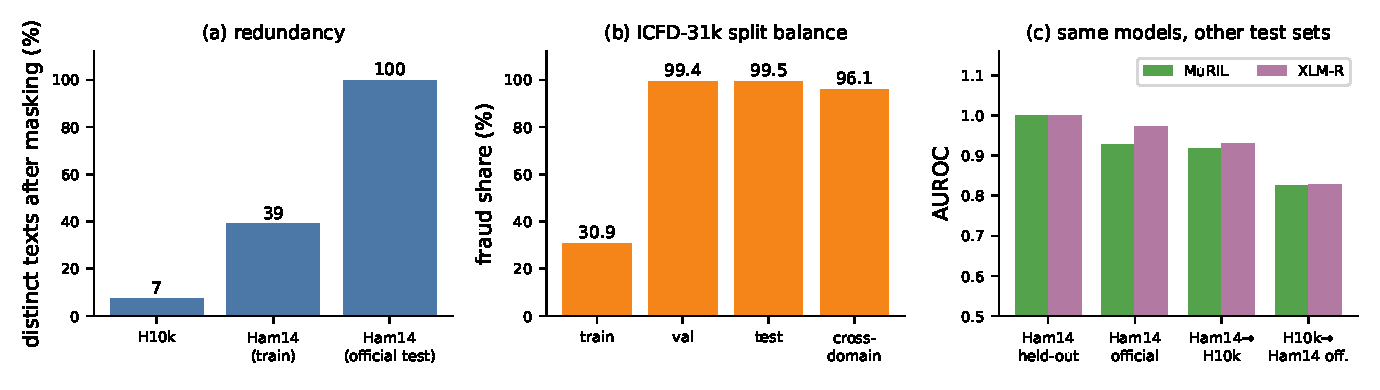
\includegraphics[width=\textwidth]{generated/fig_audit.pdf}
\caption{(a) Share of distinct texts after masking. (b) Fraud share per released ICFD-31k split. (c) AUROC of models fine-tuned on Ham14 (left three groups) or H10k (last group) on different test sets.}
\label{fig:audit}
\end{figure*}

\subsection{Real conversations from public forums are scarce}
We scanned \RdScanned{} public posts from four subreddits (r/india, r/mumbai, r/IndiaTech, r/IndianStockMarket; scanned-through dates in the released JSON), of which \RdMatched{} matched scam-related keywords. From these we extracted \RdCand{} short quoted passages with scam-related content and judged \RdVerb{} to be verbatim scam utterances, such as robocall scripts and threats, quoted by victims. All \RdVerb{} are single lines. None is multi-turn, \RdDeva{} contain Devanagari, and none has a benign counterpart, so they cannot form a test set. Most posts describe a scam in the victim's words instead of quoting it. A single reviewer made these judgments, so the count is approximate; the finding is the order of magnitude.

\section{Recommendations}
Based on these findings, we suggest that releases of scam-detection data report:
\begin{enumerate}
\item how each item was produced (collected, generated by which model, translated from which source), at item level where possible;
\item distinct templates after masking numbers and links, per language;
\item the AUROC of length/digit/link features and of any metadata fields, as a floor;
\item label balance and the meaning of the negative class in every split, with at least a few hundred negatives in test sets used to estimate false alarms, or intervals that show the uncertainty;
\item whether languages are parallel translations of one item set, and, if so, the number of independent items;
\item a hard negative set (genuine bank, police, courier and utility messages) and, where possible, a small real-world test set, even if it cannot be released as text.
\end{enumerate}
We also suggest that papers using these datasets report held-out-template, official-test and cross-dataset scores together.

\section{Limitations}
We audit what is released and documented. We could not read the full ICFD-31k paper or run its baselines, so we make no claim about its reported numbers, and we audited only the text of INDICA, not its audio. Template masking is conservative and our shortcut baselines are simple, so they understate redundancy and shortcuts. The India and China marker lists are heuristics. The encoders are base-size models, trained briefly with default settings; the zero-shot H10k-to-other-language tests are crude. The Reddit judgments come from one reviewer, and the archive and keywords may miss relevant posts. We did not evaluate large language models. Our results say nothing about real-world performance of any system, since we have no real labeled test set.

\section{Ethics and Release}
\label{sec:ethics}
All audited datasets are public and synthetic or undocumented; we process them under their stated licenses and release only scripts and aggregate numbers. Reddit text was read through a public research archive after Reddit's own site refused unauthenticated access, which we did not circumvent. Raw posts, usernames and links are not released or committed, and nothing quoted in this paper comes from them. The released code contains the extraction script and the counts. Fine-tuned detectors are not released. Scam scripts in the audited data are dual-use, and we reproduce none beyond short descriptions.

\section{Conclusion}
Near-perfect scores on current public Indian scam-detection datasets say more about the datasets than about the models: little distinct text, usable shortcuts, test sets with almost no negatives, and a multilingual set that translates Chinese-origin calls. A real, multi-turn, hard-negative test set in Hindi, Hinglish and Marathi remains the missing resource, and forum mining does not supply it.

\bibliographystyle{IEEEtran}
\bibliography{references}

\end{document}
